% +------------------------------------------------------------------------+
% | Reference manual page: Poisson_reconstruction_function.tex
% +------------------------------------------------------------------------+
% | 07.09.2007   Pierre Alliez, Laurent Saboret, Gael Guennebaud
% | Package: Surface_reconstruction_3
% |
\RCSdef{\RCSPoissonreconstructionfunctionRev}{$Id$}
\RCSdefDate{\RCSPoissonreconstructionfunctionDate}{$Date$}
% |
\ccRefPageBegin
%%RefPage: end of header, begin of main body
% +------------------------------------------------------------------------+


\begin{ccRefClass}{Poisson_reconstruction_function<GeomTraits, ReconstructionTriangulation_3>}

%% \ccHtmlCrossLink{}     %% add further rules for cross referencing links
%% \ccHtmlIndexC[class]{} %% add further index entries

\ccDefinition

% Insert image poisson.jpg/eps
\begin{center}
    \label{Surface_reconstruction_3-fig-poisson}
    % Image
    \begin{ccTexOnly}
        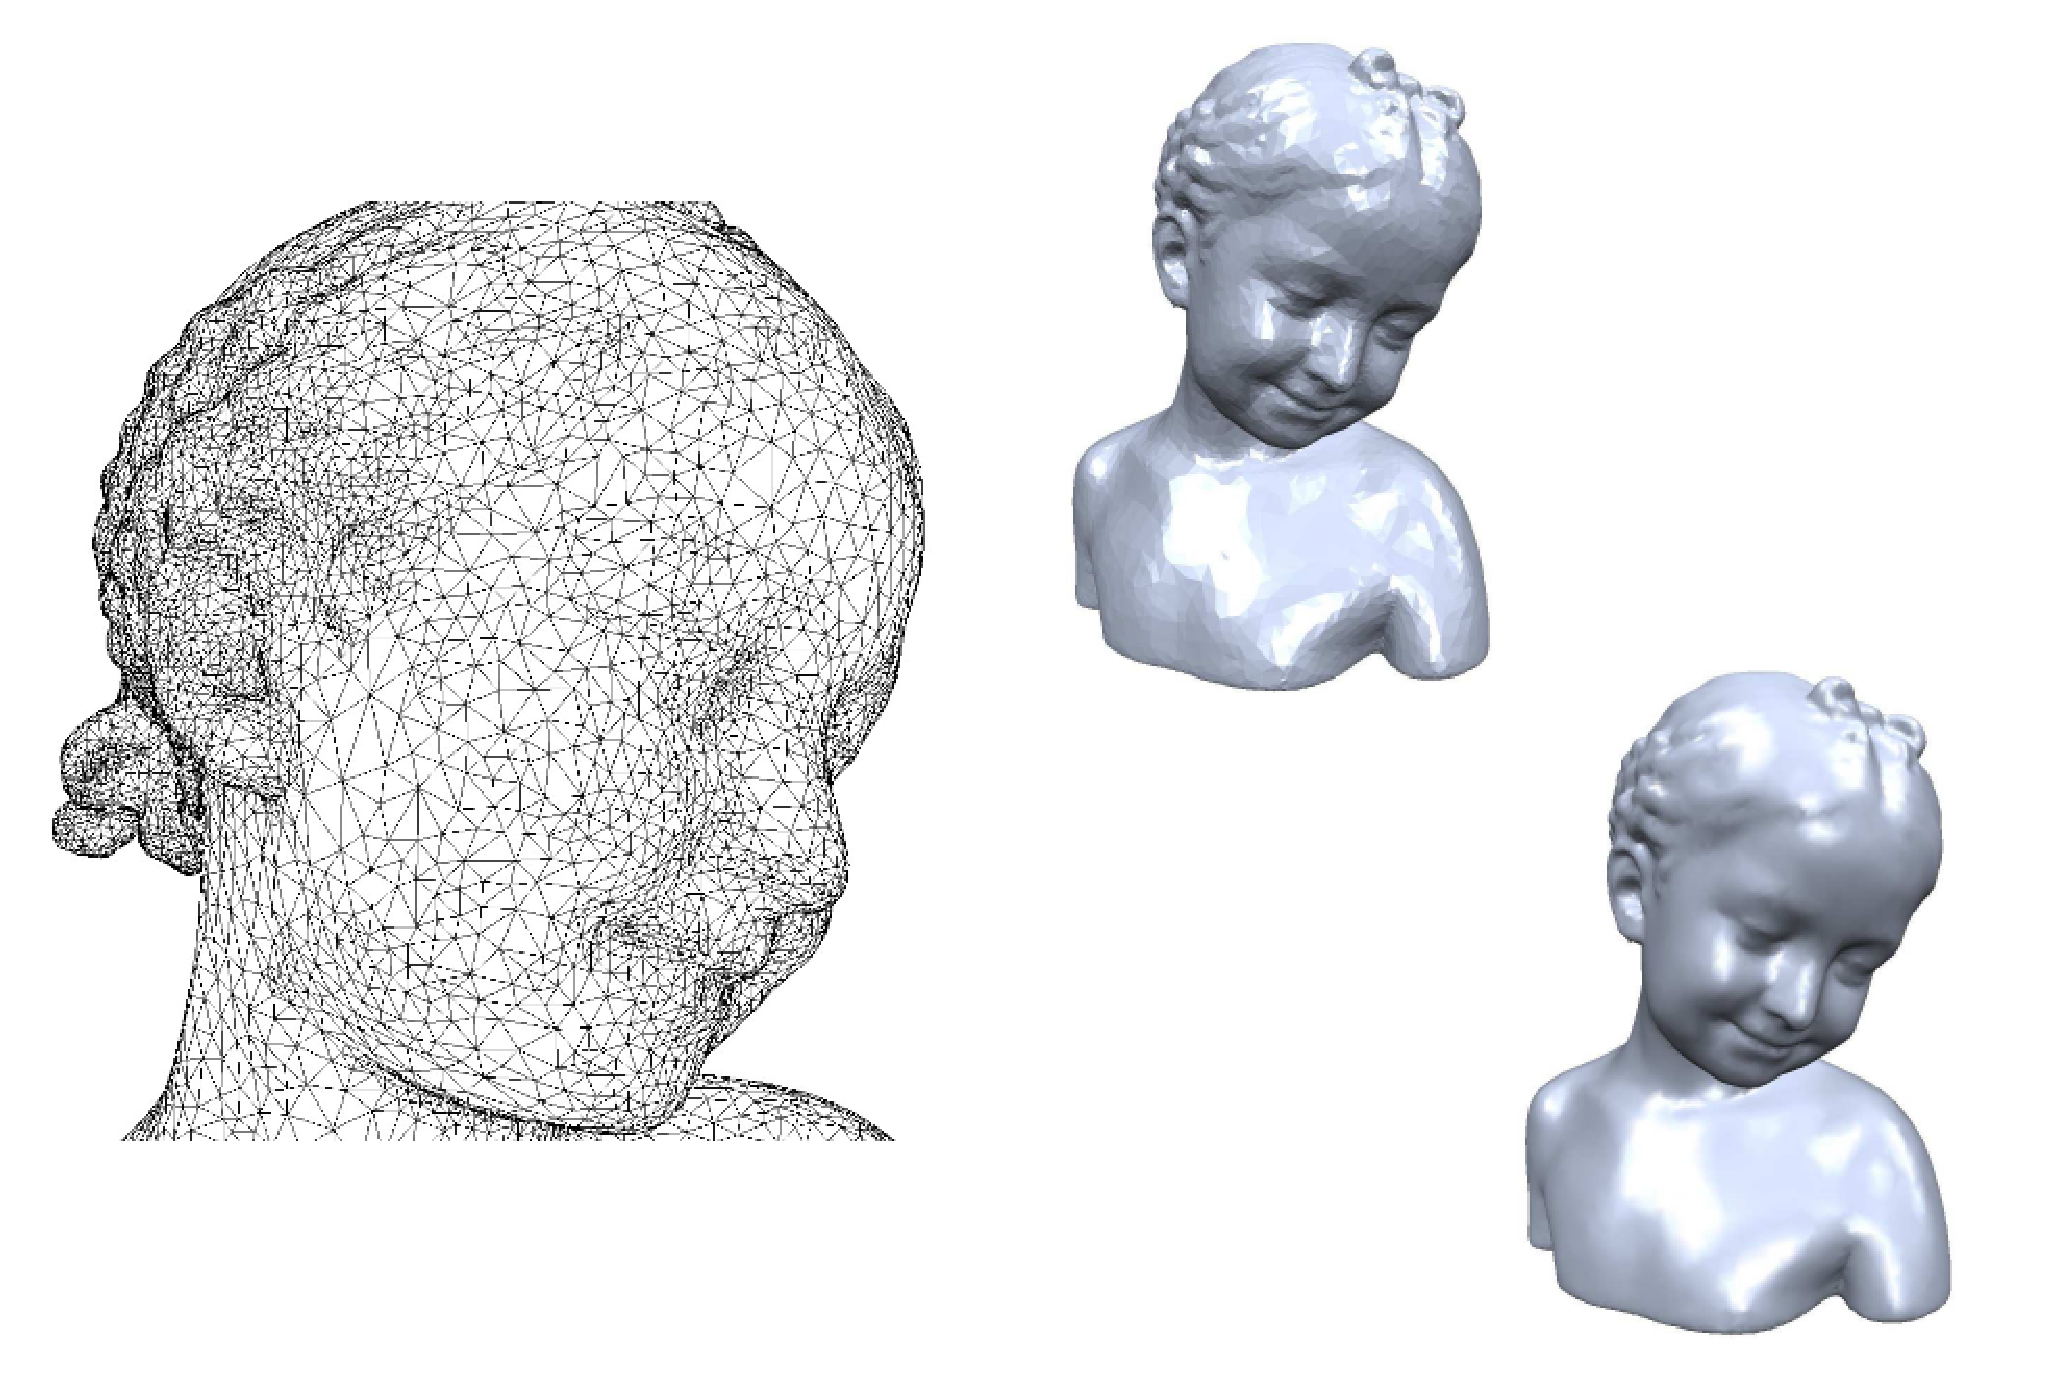
\includegraphics[width=0.7\textwidth]{Surface_reconstruction_3/poisson} % omit .eps suffix
    \end{ccTexOnly}
    \begin{ccHtmlOnly}
        <img width="70%" border=0 src="../Surface_reconstruction_3/poisson.jpg"><P>
    \end{ccHtmlOnly}
    % Title
    \begin{figure}[h]
        \caption{Poisson reconstruction}
    \end{figure}
\end{center}

Kazhdan, Bolitho and Hoppe introduced the Poisson Surface Reconstruction algorithm \cite{Kazhdan06}. Given a set of 3D points with oriented normals (denoted oriented points in the sequel) sampled on the boundary of a 3D solid, this method solves for an approximate indicator function of the inferred solid, whose gradient best matches the input normals. The output scalar function, represented in an adaptive octree, is then iso-contoured using an adaptive marching cubes. \cgal\ implements a variant of this algorithm which solves for a piecewise linear function on a 3D Delaunay triangulation instead of an adaptive octree. 

% The section below is automatically generated. Do not edit!
%START-AUTO(\ccDefinition)

\ccc{Poisson_reconstruction_function} computes an indicator function f() piecewise-linear over the tetrahedra. We solve the Poisson equation Laplacian(f) = divergent(normals field) at each vertex of the triangulation via the TAUCS sparse linear solver. One vertex must be constrained.

%END-AUTO(\ccDefinition)

% The section below is automatically generated. Do not edit!
%START-AUTO(\ccInclude)

\ccInclude{CGAL/Poisson_reconstruction_function.h}

%END-AUTO(\ccInclude)

\ccParameters

The full template declaration is:

% The section below is automatically generated. Do not edit!
%START-AUTO(\ccParameters)

template$<$  \\
class Gt,   \\
class \ccc{ReconstructionTriangulation_3}$>$   \\
class \ccc{Poisson_reconstruction_function};

\ccCommentHeading{Parameters}
\begin{description}
\item \ccc{Gt}: Geometric traits class \item \ccc{ReconstructionTriangulation_3}: 3D Delaunay triangulation, model of \ccc{ReconstructionTriangulation_3} concept. \end{description}

%END-AUTO(\ccParameters)

\ccIsModel

% The section below is automatically generated. Do not edit!
%START-AUTO(\ccIsModel)

Model of the ImplicitFunction concept.

%END-AUTO(\ccIsModel)

\ccHeading{Design Pattern}

% The section below is automatically generated. Do not edit!
%START-AUTO(\ccHeading{Design Pattern})

A model of ImplicitFunction is a Strategy \cite{cgal:ghjv-dpero-95}: it implements a strategy of surface mesh reconstruction.

%END-AUTO(\ccHeading{Design Pattern})

\ccTypes

% The section below is automatically generated. Do not edit!
%START-AUTO(\ccTypes)

\ccNestedType{Triangulation}
{
}
\ccGlue
\ccNestedType{Geom_traits}
{
Kernel's geometric traits.
}
\ccGlue
\ccNestedType{FT}
{
}
\ccGlue
\ccNestedType{Point}
{
}
\ccGlue
\ccNestedType{Vector}
{
}
\ccGlue
\ccNestedType{Iso_cuboid}
{
}
\ccGlue
\ccNestedType{Sphere}
{
}
\ccGlue
\ccNestedType{Point_with_normal}
{
Model of \ccc{PointWithNormal_3}.
}
\ccGlue
\ccNestedType{Normal}
{
Model of \ccc{Kernel::Vector_3} concept.
}
\ccGlue

%END-AUTO(\ccTypes)

\ccCreation
\ccCreationVariable{fct}  %% variable name for \ccMethod below

% The section below is automatically generated. Do not edit!
%START-AUTO(\ccCreation)

\ccConstructor{Poisson_reconstruction_function(Triangulation& pdt);}
{
Create a Poisson indicator function f() piecewise-linear over the tetrahedra of pdt. If pdt is empty, create an empty implicit function.
\ccCommentHeading{Parameters}
\ccc{pdt}: \ccc{ReconstructionTriangulation_3} base of the Poisson indicator function. 
}
\ccGlue
\ccConstructor{template<class InputIterator> Poisson_reconstruction_function(Triangulation& pdt, InputIterator first, InputIterator beyond);}
{
Create an implicit function from a point set. Insert the first...beyond point set into pdt and create a Poisson indicator function f() piecewise-linear over the tetrahedra of pdt.
\ccPrecond the value type of InputIterator must be convertible to \ccc{Point_with_normal}.
\ccCommentHeading{Parameters}
\begin{description}
\item \ccc{pdt}: \ccc{ReconstructionTriangulation_3} base of the Poisson indicator function. \item \ccc{first}: First point to add. \item \ccc{beyond}: Past-the-end point to add. \end{description}
}
\ccGlue

%END-AUTO(\ccCreation)

\ccOperations

% The section below is automatically generated. Do not edit!
%START-AUTO(\ccOperations)

\ccMethod{template<class InputIterator> int insert(InputIterator first, InputIterator beyond);}
{
Insert points.
\ccPrecond the value type of InputIterator must be convertible to \ccc{Point_with_normal}.
\ccCommentHeading{Parameters}
\begin{description}
\item \ccc{first}: First point to add. \item \ccc{beyond}: Past-the-end point to add. \end{description}
\ccCommentHeading{Returns} the number of inserted points.
}
\ccGlue
\ccMethod{void clear();}
{
Remove all points.
}
\ccGlue
\ccMethod{Triangulation& triangulation();}
{
Get embedded triangulation.
}
\ccGlue
\ccMethod{const Triangulation& triangulation() const;}
{
}
\ccGlue
\ccMethod{Iso_cuboid bounding_box() const;}
{
Get the surface's bounding box.
}
\ccGlue
\ccMethod{Sphere bounding_sphere() const;}
{
Get the surface's bounding sphere.
}
\ccGlue
\ccMethod{Sphere region_of_interest() const;}
{
Get the region of interest, ignoring the outliers. This method is used to define the OpenGL arcball sphere.
}
\ccGlue
\ccMethod{bool compute_implicit_function();}
{
You should call \ccc{compute_implicit_function}() once when points insertion is over. It computes the Poisson indicator function f() at each vertex of the triangulation by:\begin{itemize}
\item applying a Delaunay refinement to define the function inside and outside the surface.\item solving the Poisson equation Laplacian(f) = divergent(normals field) at each vertex of the triangulation via the TAUCS sparse linear solver. One vertex must be constrained.\item shifting and orienting f() such that f() = 0 on the input points, and f() $<$ 0 inside the surface.\end{itemize}
Return false on error.
}
\ccGlue
\ccMethod{void average_spacing_avg_knn_sq_distance_3();}
{
}
\ccGlue
\ccMethod{unsigned int delaunay_refinement(FT radius_edge_ratio_bound, FT cell_radius_bound, unsigned int max_vertices, FT enlarge_ratio);}
{
Delaunay refinement (break bad tetrahedra, where bad means badly shaped or too big). The normal of Steiner points is set to zero. Return the number of vertices inserted.
\ccCommentHeading{Parameters}
\begin{description}
\item \ccc{radius_edge_ratio_bound}: radius edge ratio bound (ignored if zero) \item \ccc{cell_radius_bound}: cell radius bound (ignored if zero) \item \ccc{max_vertices}: number of vertices bound \item \ccc{enlarge_ratio}: bounding box enlarge ratio \end{description}
}
\ccGlue
\ccMethod{unsigned int delaunay_refinement_shell(FT size_shell, FT sizing, unsigned int max_vertices);}
{
}
\ccGlue
\ccMethod{void extrapolate_normals();}
{
Extrapolate the normals field: compute null normals by averaging neighbor normals.
}
\ccGlue
\ccMethod{FT gaussian_function(FT sigma, FT distance);}
{
}
\ccGlue
\ccMethod{int extrapolate_normals_using_gaussian_kernel();}
{
Extrapolate the normals field. Return the number of normals computed.
}
\ccGlue
\ccMethod{bool solve_poisson(double lambda, double * duration_assembly, double * duration_factorization, double * duration_solve, bool is_normalized = false);}
{
Poisson reconstruction. Return false on error.
}
\ccGlue
\ccMethod{void SaveAsMeshFile();}
{
}
\ccGlue
\ccMethod{FT set_contouring_value(FT contouring_value);}
{
Shift and orient the implicit function such that:\begin{itemize}
\item the implicit function = 0 for points / f() = \ccc{contouring_value},\item the implicit function $<$ 0 inside the surface.\end{itemize}
Return the minimum value of the implicit function.
}
\ccGlue
\ccMethod{FT f(const Point& p) const;}
{
Evaluate implicit function for any 3D point.
}
\ccGlue
\ccMethod{FT operator()(const Point& p) const;}
{
[ImplicitFunction interface]
Evaluate implicit function for any 3D point.
}
\ccGlue
\ccMethod{Point get_inner_point() const;}
{
Get point inside the surface.
}
\ccGlue
\ccMethod{FT average_value_at_input_vertices() const;}
{
Get average value of the implicit function over input vertices.
}
\ccGlue
\ccMethod{FT median_value_at_input_vertices() const;}
{
Get median value of the implicit function over input vertices.
}
\ccGlue
\ccMethod{FT min_value_at_input_vertices() const;}
{
Get min value of the implicit function over input vertices.
}
\ccGlue
\ccMethod{FT max_value_at_input_vertices() const;}
{
Get max value of the implicit function over input vertices.
}
\ccGlue
\ccMethod{FT median_value_at_convex_hull() const;}
{
Get median value of the implicit function over convex hull vertices.
}
\ccGlue
\ccMethod{FT average_value_at_convex_hull() const;}
{
Get average value of the implicit function over convex hull vertices.
}
\ccGlue

%END-AUTO(\ccOperations)

\ccSeeAlso

\ccRefIdfierPage{CGAL::Reconstruction_triangulation_3<GeomTraits, TriangulationDataStructure_3>}  \\
\ccRefIdfierPage{CGAL::Reconstruction_cell_base_3<GeomTraits, TriangulationCellBase_3>}  \\
\ccRefIdfierPage{CGAL::Reconstruction_vertex_base_3<GeomTraits, TriangulationVertexBase_3>}  \\
\ccRefIdfierPage{CGAL::APSS_reconstruction_function<GeomTraits>}  \\

\ccExample

\ccIncludeExampleCode{Surface_reconstruction_3/poisson_reconstruction_example.cpp}

\end{ccRefClass}

% +------------------------------------------------------------------------+
%%RefPage: end of main body, begin of footer
\ccRefPageEnd
% EOF
% +------------------------------------------------------------------------+

